\textbf{Cas d'utilisation:} Payer avec carte blue

\textbf{Acteur primaire:} Le conducteur

%\textbf{Acteur support:}

\textbf{Pré-condition: } la borne affiche le montant

 
%\textbf{Post-condition: } 

\textbf{Scenario primaire: } \\
    \textbf{1.}Le conducteur insère sa carte bancaire pour payer. \\ %La borne détecte si la carte est volée
    \textbf{2.} La borne accepte le paiement \\
    \textbf{3.} Le conducteur récupère sa carte.\\

\textbf{Variantes:}\\
    %\textbf{1a.} Le conducteur insère une carte volée, un technicien est appelé.
    \textbf{2a.} Le conducteur insère une carte invalide, la borne rend la carte et un technicien est appelé\\
    
%\textbf{Décomposition des cas d'utilisation:} 
%\begin{figure}[h]
 %   \centering
  %  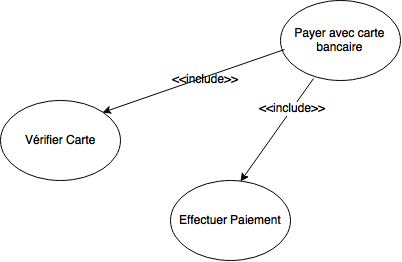
\includegraphics[scale=0.7]{02_Desenvolvimento/TD2/images/CarteBleueCockburn.png}
   % \caption{Décomposition des cas d'utilisation: Payer avec carte blue}
%\end{figure}
